\section{設計} \label{sec:design}

\sysname は,前述した設計上の課題に対するソフトウェアレベルの解決策を提供する.
コンポーネント単位で効率的に Unikernel を若返らせるために,
\sysname は各コンポーネントごとの専用のスレッドを用意し,
コンポーネントの再起動が
他のコンポーネントの実行に影響を与えるのを防ぐ.
再起動したコンポーネントが他のコンポーネントの動作状態に影響を与えるのを防ぐため,
\sysname は,ログの再生時に,再起動したコンポーネントをカプセル化する.
また,\sysname は,コンポーネント初期化後に取得したコンポーネントのメモリスナップショットを使用し,
選択的に対象のコンポーネントの状態を変化させる関数のみを実行する.


\subsection{マルチスレッド Unikernel コンポーネント}

Unikernel をコンポーネント単位で若返えらせるために,
Unikernel コンポーネントの実行について考慮する必要がある.
Unikernel がライブラリのように動作するため,
各コンポーネントはその機能を呼び出すスレッドコンテキストによって実行される.
Unikernel にリンクされたアプリケーションのスレッドがファイルを開くことを要求すると,
そのコンテキストはファイルシステム関連のコンポーネントを実行する.
単純なアプローチでは,スレッドコンテキストが対象のコンポーネントに到達したときに
そのコンポーネントを若返らせる.
この方法では,その実行に直接影響を与えるため,現在のコンテキストに関係ないコンポーネントを若返らせることができなくなる.
たとえば,Unikernel にリンクされたアプリケーションがファイル関連の処理を実行している間は,
ネットワークコンポーネントを若返らせることができない.

この問題を解決するために,
\sysname はすべてのコンポーネントに専用のスレッドを割り当てて,
メッセージパッシング方式で相互に交流する.
この方式は,アプリケーションのコンテキストに対して, \sysname のコンポーネントの透過的な再起動を可能にする.
たとえば,\sysname は,アプリケーションスレッドが使用していないコンポーネントを若返らせることができ,
再起動がアプリケーションの挙動に影響を与えるのを防ぐ.
そして,再起動されたコンポーネントの動作状態を復元することで,
\sysname にリンクされたアプリケーションが再起動に渡って動作を継続し続けることができる.

書き込み可能な領域(データ領域と BSS 領域,ヒープ領域)が,それぞれ,\sysname のコンポーネントごとに分割,割り当てられる.
コンポーネントに実装されている関数は,
呼び出し元コンポーネントのスレッドではなく,
自身に割り当てられている専用のスレッドによって,割り当てられた領域内部で実行される.
各スレッドは,
他のコンポーネントの関数の引数を呼び出し先のコンポーネントに渡すことにより,
その関数を呼び出し,関数の実行には,コンポーネントごとのメモリ領域が使われる.
通常の Unikernel では,アプリケーションがファイルを開くために,VFS (仮想ファイルシステム)のコンポーネントが公開する \textbf{open()} を呼び出す際には,
アプリケーションのスレッドコンテキストが VFS コンポーネントの \textbf{open()} へとジャンプする.
一方で, \sysname にリンクされたアプリケーションがファイルを開くには,
アプリケーションのスレッドが \textbf{open()} の引数を VFS コンポーネントに渡し,
VFS コンポーネントのスレッドが \textbf{open()} を実行する.
\sysname が引数を取り出すために,コンポーネントによって公開されたインタフェースをフックし,
呼び出し先のコンポーネントのメモリにその引数をコピーする.
関数の実行中に参照される引数は,
呼び出し元のコンポーネントのメモリにあるものではなく,
自身のメモリ上の複製されたものである.


\subsection{コンポーネントの再起動}


\sysname のコンポーネントの再起動は,
ソフトウェア若化のほかに
クラッシュやハングアップからのリカバリにも使われる.
ソフトウェア若化~\cite{HuangEtAl-rejuvenation,CotroneoEtAl-rejuvenation-survey,CotroneoEtAl-Surv14}の実現のために,
\sysname は一定の時間間隔でコンポーネントの再起動を繰り返す.
一方,クラッシュやハングアップに対しては,
それらのフォルトが発生した後に,
リアクティブに対象のコンポーネントの再起動を行い,動作を再開させる.
クラッシュは CPU トラップ時のエラーコードによって検出し,
ハングアップは関数実行に対してタイムアウトを設けることで検出する.


Unikernel のコンポーネント単位の再起動において,
対象のコンポーネントの動作状態に注意を払う.
Unikernel では,汎用 OS で動作するアプリケーションをビルドするために,
いくつもの状態を持たないコンポーネントを構成することがある.
たとえば,Unikernel にはユーザプロセスが存在しないため,
\textbf{get\_pid()} や \textbf{fork()}
といった関数が 0 や -1 などの定数を返すだけの処理として実装されることで,
これらを実装するコンポーネントが状態を持たないことがある.
コンポーネントが状態を持たない場合は,
コンポーネントスレッドのコンテキストの初期化によって再起動を行う.
状態を持たないコンポーネントは経年劣化をしないため,
そのコンポーネントで発生するフォルトは
コーナーケースのソフトウェアバグなどに起因する一時的なものである傾向があり,
コンポーネント単位での再起動によるリカバリが有効である~\cite{BhatEtAl-OSIRIS, LiEtAl-TxIPC}.

一方,
ファイルシステムやネットワークのような多くの OS サブシステムが状態を持つが,
それらの状態持つ Unikernel コンポーネントの再起動に渡って,
アプリケーションと他のコンポーネントを継続して動作させることができない.
たとえば,ファイルオフセットを保持する VFS コンポーネントを再起動させると,
ファイルオフセットが 0 に初期化されるため,
再起動後のアプリケーションのファイル操作を正しく行えなくなる.
ソフトウェア若化の観点から,
対象のコンポーネントのメモリスナップショットを再起動の直前に取得し,
動作状態を復元するのは意味がない.
なぜなら,メモリリークやディスクリプタリーク,メモリフラグメンテーションを含む
古くなったメモリイメージが再作成されるからである.

\begin{figure}[t]
    \centering
    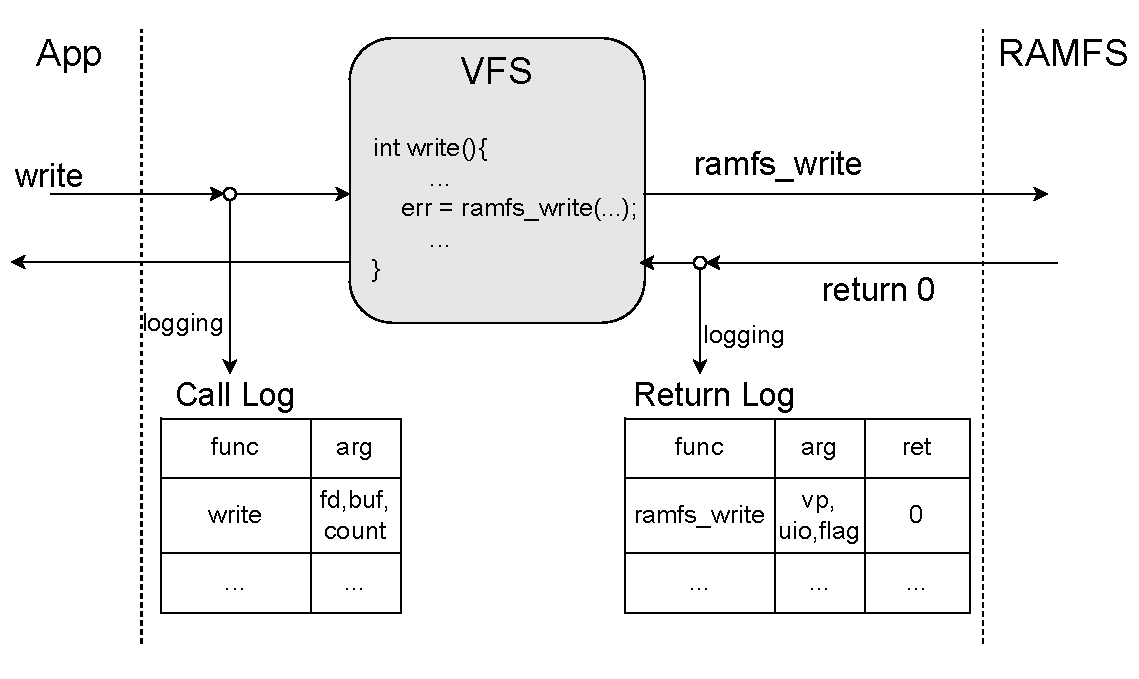
\includegraphics[width=\linewidth]{img/logging.pdf}
    \vspace{-5mm}
    \caption{コンポーネント間のインタラクションのロギング}
    \label{fig:logging}
\end{figure}

\begin{figure}[t]
    \centering
    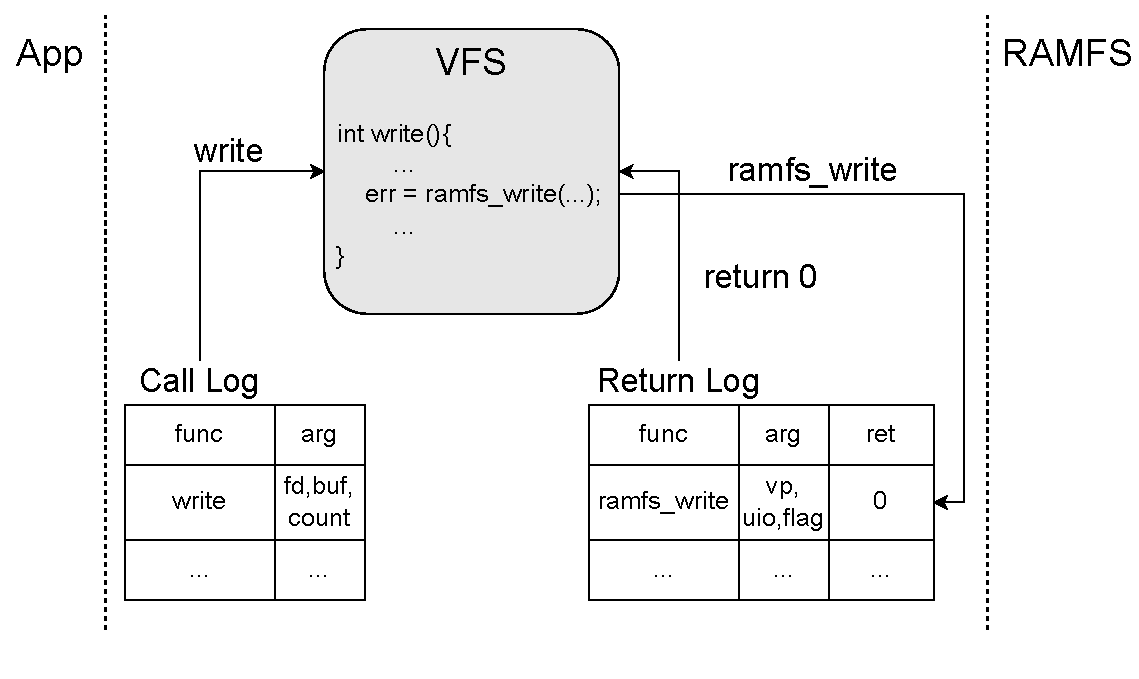
\includegraphics[width=\linewidth]{img/playlog.pdf}
    \caption{コンポーネントの復元のためのログの再生}
    \label{fig:restoration}
\end{figure}

状態を持つコンポーネントの再起動によって生じる不整合を防ぐため,
再起動の後に状態を持つコンポーネントの動作状態を復元する.
復元のために,\sysname は,他のコンポーネントからの対象の関数に対する関数呼び出しを記録し,
再起動の後にコンポーネントのログを再生する.
図\ref{fig:logging}は,\sysname のコンポーネント間のインタラクションのロギングを表している.
他のコンポーネントに対して透過的に再起動したコンポーネントの動作状態を復元するために,
{\sysname} はコンポーネントが公開するインタフェースをフックし,関数呼び出しを記録した後,値を返す.
再起動前に実行されたすべての関数を再実行するわけではない.
復元時間の短縮およびメモリリークやメモリフラグメンテーションのような老化関連のバグによるエラー状態の再現を防ぐため,
\sysname は選択的に関数を呼び出す.
\sysname は,再起動の直前の状態を復元するのに必要な関数のみを呼び出す.
具体的には,ファイル状態の読み出し(\textbf{fstat()} 関連の関数)のようなコンポーネントの状態を変更しない関数は,
呼び出されない.
また,\sysname はすでに閉じられたファイルへの操作といった
コンポーネントの現在の状態を生成しない関数は再実行しない.
ログの再生によって,再起動前の動作状態を復元することができないデータ構造には,
再起動の直前に復元不可能なデータを退避し,再起動後の同じデータ構造にそれを設定することで,動作状態を復元する.
たとえば,ネットワークコンポーネントにおける TCP 通信の状態復元をログの再生によって行うことはできない.
TCP 通信では,ACK 番号やシーケンス番号などのサーバ,クライアント間のインタラクションによって維持される状態があり,
どちらか一方のみを再起動した場合にサーバ,クライアント間で不整合が生じる.


さらに,\sysname では,他のコンポーネントの関数を呼び出した際の戻り値のロギングも行う.
記録した関数の戻り値は,対象のコンポーネントの状態のみを復元するのに使われる.
ログの再生による関数の実行のための単純なアプローチは,
記録されている引数で,ただ,関数を実行することである.
しかし,このアプローチでは,
再起動したコンポーネントの動作状態を復元している間に,
他のコンポーネントの関数を呼び出すことで,
そのコンポーネントの状態を変えてしまう.
これらの状態の変化は,通常の操作ではなく,復元の操作によって引き起こされるため,
動作中のアプリケーションと対応するコンポーネントとの不整合が生じる.
復元中に再起動したコンポーネントから他のコンポーネントに状態を変化させる関数の呼び出しを防ぐために,
他のコンポーネントの関数を呼び出すのではなく,ログに記録された値を関数の戻り値として返す.
図\ref{fig:restoration}は,\sysname のコンポーネントの状態復元の概要である.
コンポーネントの再起動の後に,\sysname は自身の状態を復元するための関数をコンポーネントに実行させる.
その際,再起動前にログに記録した他のコンポーネントの関数呼び出しの戻り値を利用させることで,
その実行による他のコンポーネントの動作状態の変化を防ぐ.



\subsection{チェックポイントベースの再起動}

シャットダウンやブート処理を行う
通常のコンポーネントの再起動は,
コンポーネント単位の再起動には適していない.
その処理は,他のコンポーネントの関数呼び出しやハードウェアの操作を含み,
コンポーネントやハードウェアの動作状態を変化させてしまう.
たとえば,RAM ファイルシステム上のメモリの読み書きを行う RAMFS コンポーネントは,
シャットダウンの段階でファイルシステム内のすべての内容を消去してしまう.

この問題を解決するために,
\sysname は,
phase-based reboot~\cite{YamakitaEtAl-PBR}のアイデアを借りて,
初期化直後のコンポーネントのメモリイメージを利用する.
この phase-based reboot では,起動段階でのシステムのメモリイメージを復元することによる
再起動の効果を獲得する.
\sysname は,コンポーネント単位のチェックポイントメカニズムを提供し,
初期化されたコンポーネントのメモリスナップショットを取得する.
前述したように,
コンポーネントの再起動において,
\sysname はそのメモリスナップショットの復元とログの再生を実行する.


\subsection{Intel MPK を用いたエラー伝搬の防止}

コンポーネント間のエラー伝搬の防止には,
コンポーネントの粒度でのメモリの書き込み制限が有効である.
私たちは,コンポーネントの保護のために Intel の Memory Protection Keys (MPK)~\cite{Intel-Manual2023}
を使用する.
MPK は,CPU の命令セットアーキテクチャの拡張であり,
メモリのアクセス権限を細かい粒度で高速に制御することができる.
その有用性から,
MPK を用いたセキュリティメカニズム
がいくつか提案されている\cite{ParkEtAl-libmpk,HedayatiEtAl-Hodor,SchrammelEtAl-Donky,SartakovEtAl-ASPLOS21,LefeuvreEtAl-FlexOS}.
しかし,本研究は Unikernel の \rr をテーマとしており,
コンポーネントのエラー伝搬防止のためだけに MPK を使用し,
Unikernel への攻撃を想定しない.
また,Unikernel がリンクするアプリケーションとすべての Unikernel コンポーネントが同じ特権モードで動作し,
MPK の制御下にあるため,
特権モードの違いに起因するエラー伝搬~\cite{ConnorEtAl-PKUPitfalls,VoulimeneasEtAl-CERBERUS,SchrammelEtAl-Jenny}
が発生することもない.


MPK では,ページ単位でメモリへの読み書きを制限することができる.
各ページテーブルエントリ(PTE)には 4 ビットの保護キーが設定され,
CPU コアごとの PKRU レジスタには各保護キーの設定されたページへのアクセス権限が保存されている.
メモリアクセスの度に,
メモリ管理ユニット(MMU)が対象のページの保護キーで PKRU レジスタに保存されているアクセス権限を参照し,
権限がない場合にはページフォルトが発生する.
保護キーの上限を拡張するような研究\cite{ParkEtAl-libmpk,ChenEtAl-Shreds,GuEtAl-EPK}も存在するが,
汎用的なアプリケーションである SQLite,Redis,Nginx の動作に必要なコンポーネント数はその上限を下回るため,
現状では,それらのメカニズムの導入を考えていない.

\sysname では,MPK の保護キーを各コンポーネントに割り当てて,
コンポーネント外部からの書き込みを制限することで,
コンポーネント粒度でのメモリ保護を実現する.
コンポーネントスレッドは,自身の実行するコンポーネント以外のコンポーネントのデータへの書き込みができなくなり,
ほとんどのエラー伝搬を防ぐことができる.
このメカニズムで防ぐことができないエラー伝搬については,\ref{sec:disc}章で述べる.


